\documentclass[11pt]{article}

\usepackage[tmargin = 2cm, lmargin=2cm, rmargin = 3cm, bmargin = 2cm]{geometry} % set the margins to 1in on all sides
\usepackage{MyMainPreamble}
\usepackage{relsize}


\let\Im\undefined
\DeclareMathOperator{\Im}{Im}
\let\Re\undefined
\DeclareMathOperator{\Re}{Re}
\DeclareMathOperator{\End}{End}
\let\mod\undefined
\newcommand{\mod}{\hspace{3pt}\text{mod}\hspace{2pt}}
%\newcommand{\mathbf}[1]{\mathbf{#1}}
%END_FOLD

\allowdisplaybreaks

\renewcommand{\H}{\mathcal{H}}
\newcommand{\G}{\mathcal{G}}
\newcommand{\gtp}{\otimes_{\text{gr}}}

\lhead{\leftmark\newline\rightmark}
\chead{}
\rhead{}
\title{Documentation For Quantum Haze}
\author{By Quintessence}

\begin{document}
  \maketitle
  \begin{abstract}
    We use a Bose-Hubbard model, GPT3 and Dalle-2 to generate an illustrated story of Mr Quanta's eventful evening. 
  \end{abstract}
  \tableofcontents
  \section{Overview}
    In Quantum Haze, we help Mr Quanta recall his eventful evening. This is done by modeling his activities as a quantum random walk of a single particle in a 1D Bose-Hubbard hopping model with periodic boundary conditions with each site being a possible location that Mr Quanta visited the night before. After evolving the quantum random walk, we get a superposition of single occupancy states with the amplitudes at each site informing Mr Quanta of how likely he ended up there. These results, along with the  Shannon entropy of the final state are used to generate a prompt for GPT3 to write an outline of Mr Quanta's evening. We then use these to get illustrations of his night from Dalle-2. 
  \section{The Circuit}
    In our code, we  perform a random walk by Trottterizing the Bose-Hubbard Hamiltonian and evolving a state with occupation number one. The lattice diagram for this system is given in \ref{fig:Lattice}.
    \begin{figure}[h]
      \centering
      \begin{tikzpicture}
        \node at (15:3.5cm) {$h_{i,i+1}$};
        \node at (0:3.7cm) {$\kappa_i\sigma^z_i$};
        \foreach \i in {0,30,60,...,360}{% 
        \draw (\i:3cm)--(\i+30:3cm);
        \filldraw [blue]  (\i:3cm) circle (5pt);
        }
        \filldraw [red]  (90:3cm) circle (5pt);
      \end{tikzpicture}
      \caption{The circular hopping lattice for 12 sites where $h_{i,i+1} = -J\sum\limits_{\alpha=\{x,y\}}\sigma_i^\alpha\sigma^\alpha_{i+1}$.}\label{fig:Lattice}
    \end{figure}

    This model is implemented by the quantum circuit given in figure \ref{fig:Circuit}. The Hamiltonian is number conserving, meaning that in the evolution of our system, the states should stay in the single occupancy Hilbert space. However, errors in the computer can introduce contributions from different occupancy states. In terms of the story, we consider these errors as gaps in Mr Quanta's memory that he just cannot seem to fill. 

    The starting location of the walker  (Mr Quanta) is determined by starting the system in the $\ket{0}$ state and applying $\sigma_x$ at the starting location to flip that qubit. 
    \begin{figure}[H]
      \centering
      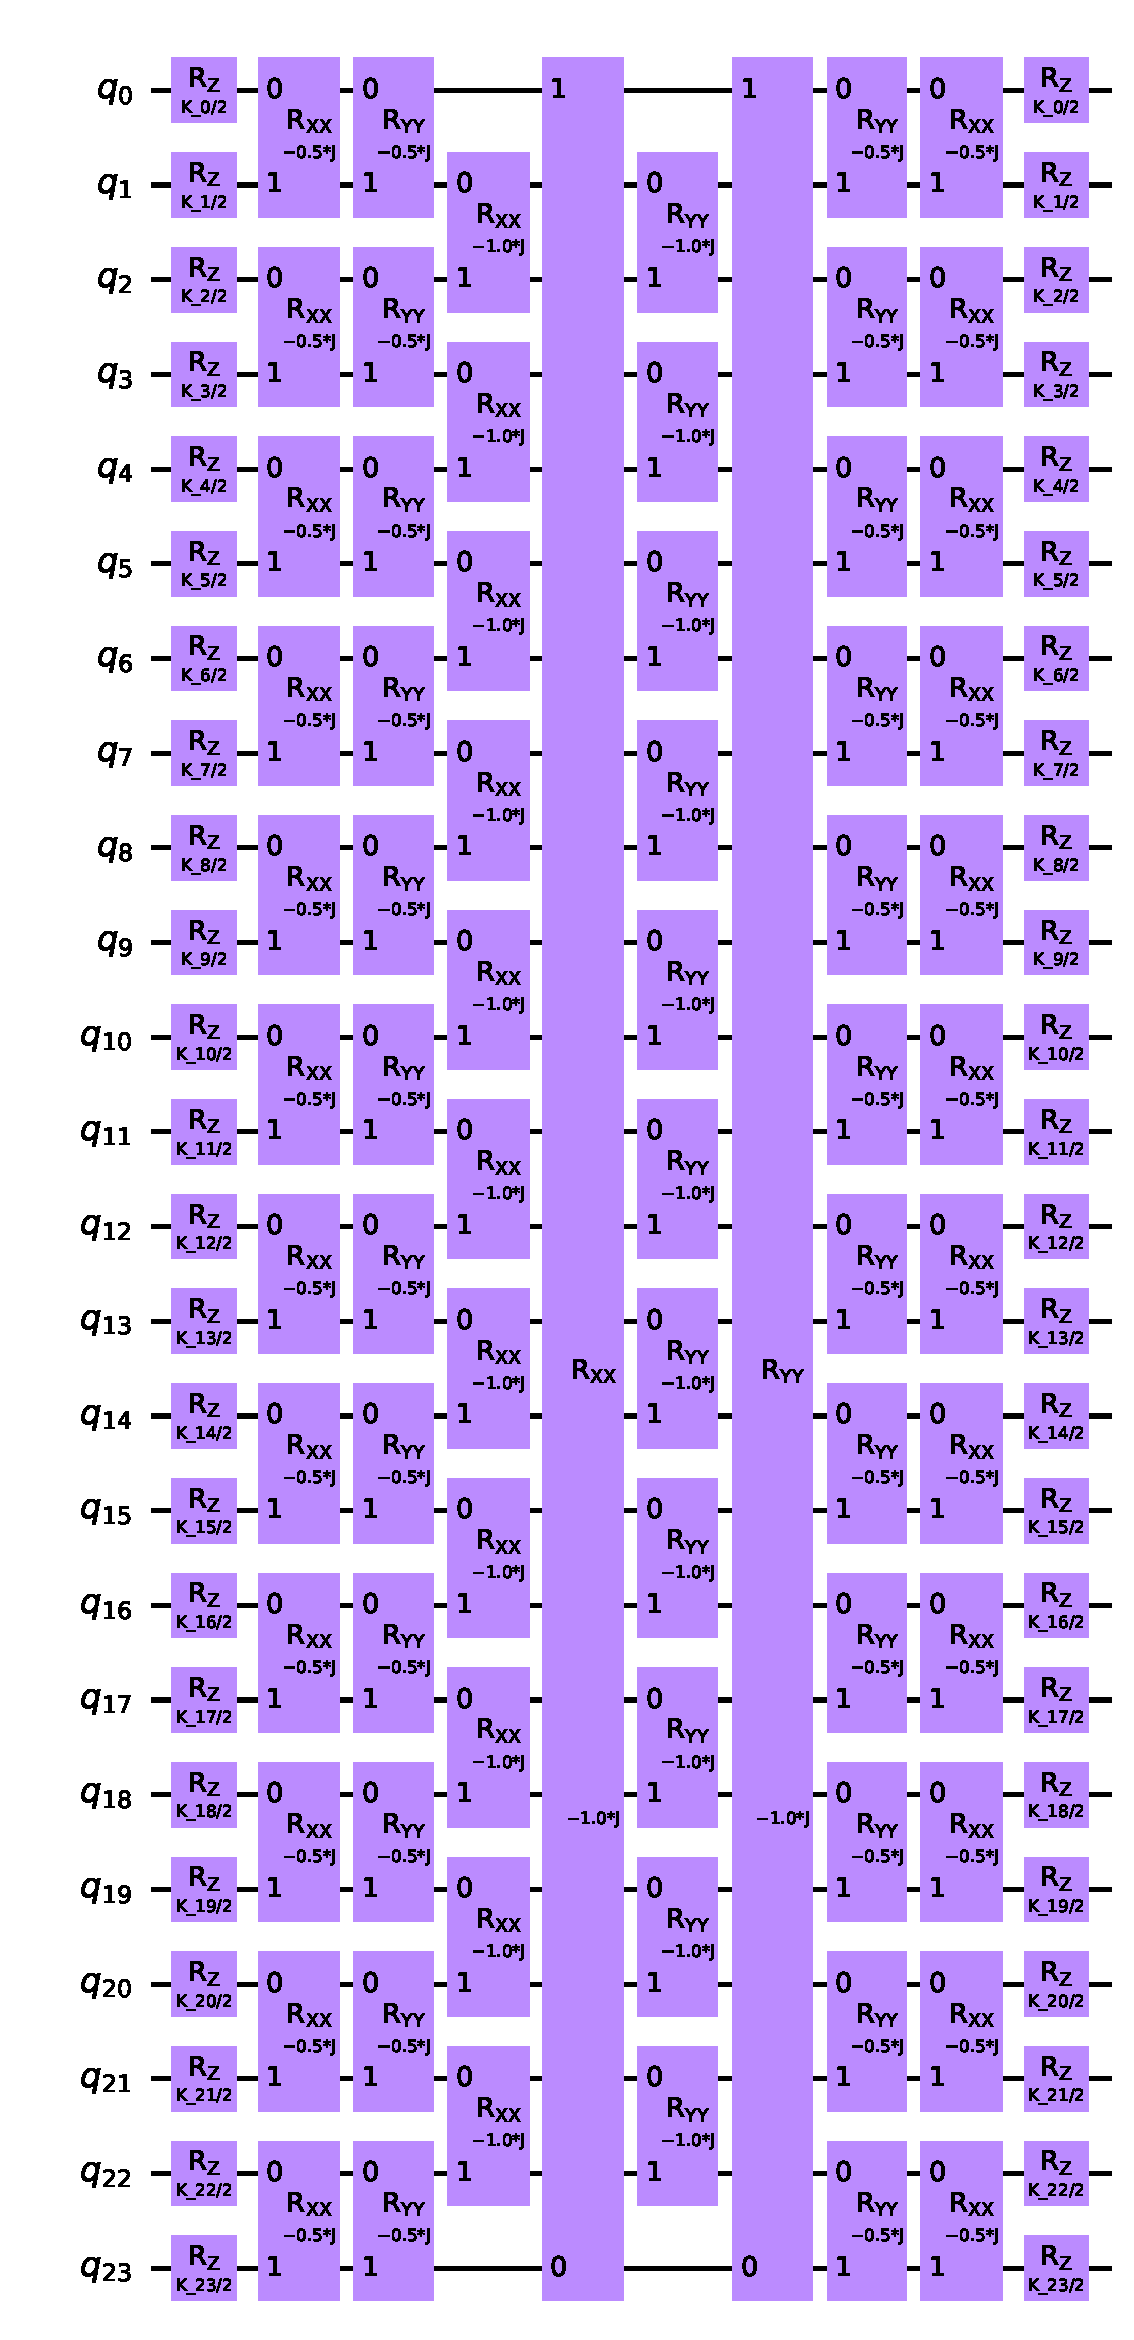
\includegraphics[scale =  0.2]{Figures/Unitary_Gate_iQuHACK23.pdf}
      \caption{A single implementation of Trottterized Hamiltonian.}\label{fig:Circuit}
    \end{figure}
    
  \section{Simulation vs Running on Hardware}
    For the simulations of the circuit, we can run as many Trotter steps as we want for our story. This is just running multiple copies of the circuit given in figure \ref{fig:Circuit}. For the hardware, we ran into the issue of non-parallelizability of the IonQ machine. With the amount of gates we have, this causes the circuit depth to grow by $8\times\text{(number of qubits)}$ per Trotter step. In our two runs, we did one with one Trotter step and another with two. For both we did 1024 shots and got unusable results.  
      

  
  \bibliography{EntanglementinSpinChains.bib}
  \bibliographystyle{plainnat}
\end{document}	
